\documentclass[11pt,twocolumn,oneside,openany,headings=optiontotoc,11pt,numbers=noenddot,final]{article}

\usepackage[a4paper]{geometry}
\usepackage[utf8]{inputenc}
\usepackage[T1]{fontenc}
\usepackage{lmodern}
\usepackage[ngerman]{babel}
\usepackage{ngerman}

\usepackage[onehalfspacing]{setspace}

\usepackage{fancyhdr}
\usepackage{fancybox}

\usepackage{rotating}
\usepackage{varwidth}

%Struktogramme
\usepackage[german,curves]{struktex}

\usepackage{pdflscape}
\usepackage{changepage}
\usepackage{graphicx}
\usepackage[bottom]{footmisc}
\usepackage{transparent}
\usepackage{graphbox}
\graphicspath{
	{Pics/PDFs/}
	{Pics/JPGs/}
	{Pics/PNGs/}
}
\usepackage{caption}
\usepackage{wrapfig}
\usepackage{marginnote}
\usepackage{tabularx}
\usepackage{dashrule}
\usepackage{soulutf8}
\usepackage{hhline}
%arydshln suppresses vertical lines in table
%\usepackage{arydshln}
\usepackage{multirow}
\usepackage{enumerate}
\usepackage[hidelinks]{hyperref}
\usepackage{listings}

\usepackage[table]{xcolor}
\usepackage{array}
\usepackage{enumitem,amssymb,amsmath}
\usepackage{interval}
\usepackage{cancel}
\usepackage{stmaryrd}
\usepackage{wasysym}
\usepackage{polynom}
\usepackage{diagbox}
\usepackage{dashrule}
\usepackage{framed}
\usepackage{mdframed}
\usepackage{karnaugh-map}
\usepackage{pdfpages}

\usepackage{blindtext}

\usepackage{eso-pic}

\usepackage{amssymb}
\usepackage{eurosym}

\usepackage[pages=some]{background}
\pagestyle{headings}
\renewcommand{\headrulewidth}{0.2pt}
\renewcommand{\footrulewidth}{0.2pt}
\newcommand*{\underdownarrow}[2]{\ensuremath{\underset{\overset{\Big\downarrow}{#2}}{#1}}}
\setlength{\fboxsep}{5pt}
\newcommand{\explainBelow}[3]{\underbrace{#1}_{\parbox{\widthof{#3}}{\footnotesize\raggedright #2}}}
\newcommand{\explainAbove}[3]{\overbrace{#1}^{\parbox{\widthof{#3}}{\footnotesize\raggedright #2}}}
\newcommand\footnoteref[1]{\protected@xdef\@thefnmark{\ref{#1}}\@footnotemark}


% Codestyle defined
\definecolor{codegreen}{rgb}{0,0.6,0}
\definecolor{codegray}{rgb}{0.5,0.5,0.5}
\definecolor{codepurple}{rgb}{0.58,0,0.82}
\definecolor{backcolour}{rgb}{0.95,0.95,0.92}
\definecolor{deepgreen}{rgb}{0,0.5,0}
\definecolor{darkblue}{rgb}{0,0,0.65}
\definecolor{mauve}{rgb}{0.40, 0.19,0.28}
\colorlet{exceptioncolour}{yellow!50!red}
\colorlet{commandcolour}{blue!60!black}
\colorlet{numpycolour}{blue!60!green}
\colorlet{specmethodcolour}{violet}

%Neue Spaltendefinition
\newcolumntype{L}[1]{>{\raggedright\let\newline\\\arraybackslash\hspace{0pt}}m{#1}}
\newcolumntype{M}{>{\centering\arraybackslash}X}
\newcommand{\cmnt}[1]{\ignorespaces}
%Textausrichtung ändern
\newcommand\tabrotate[1]{\rotatebox{90}{\raggedright#1\hspace{\tabcolsep}}}

%Intervall-Konfig
\intervalconfig {
	soft open fences
}

%Bash
\lstdefinestyle{BashInputStyle}{
	language=bash,
	basicstyle=\small\sffamily,
	backgroundcolor=\color{backcolour},
	columns=fullflexible,
	backgroundcolor=\color{backcolour},
	breaklines=true,
}
%Java
\lstdefinestyle{JavaInputStyle}{
	language=Java,
	backgroundcolor=\color{backcolour},
	aboveskip=1mm,
	belowskip=1mm,
	showstringspaces=false,
	columns=flexible,
	basicstyle={\footnotesize\ttfamily},
	numberstyle={\tiny},
	numbers=none,
	keywordstyle=\color{purple},,
	commentstyle=\color{deepgreen},
	stringstyle=\color{blue},
	emph={out},
	emphstyle=\color{darkblue},
	emph={[2]rand},
	emphstyle=[2]\color{specmethodcolour},
	breaklines=true,
	breakatwhitespace=true,
	tabsize=2,
}
%Python
\lstdefinestyle{PythonInputStyle}{
	language=Python,
	alsoletter={1234567890},
	aboveskip=1ex,
	basicstyle=\footnotesize,
	breaklines=true,
	breakatwhitespace= true,
	backgroundcolor=\color{backcolour},
	commentstyle=\color{red},
	otherkeywords={\ , \}, \{, \&,\|},
	emph={and,break,class,continue,def,yield,del,elif,else,%
		except,exec,finally,for,from,global,if,import,in,%
		lambda,not,or,pass,print,raise,return,try,while,assert},
	emphstyle=\color{exceptioncolour},
	emph={[2]True,False,None,min},
	emphstyle=[2]\color{specmethodcolour},
	emph={[3]object,type,isinstance,copy,deepcopy,zip,enumerate,reversed,list,len,dict,tuple,xrange,append,execfile,real,imag,reduce,str,repr},
	emphstyle=[3]\color{commandcolour},
	emph={[4]ode, fsolve, sqrt, exp, sin, cos, arccos, pi,  array, norm, solve, dot, arange, , isscalar, max, sum, flatten, shape, reshape, find, any, all, abs, plot, linspace, legend, quad, polyval,polyfit, hstack, concatenate,vstack,column_stack,empty,zeros,ones,rand,vander,grid,pcolor,eig,eigs,eigvals,svd,qr,tan,det,logspace,roll,mean,cumsum,cumprod,diff,vectorize,lstsq,cla,eye,xlabel,ylabel,squeeze},
	emphstyle=[4]\color{numpycolour},
	emph={[5]__init__,__add__,__mul__,__div__,__sub__,__call__,__getitem__,__setitem__,__eq__,__ne__,__nonzero__,__rmul__,__radd__,__repr__,__str__,__get__,__truediv__,__pow__,__name__,__future__,__all__},
	emphstyle=[5]\color{specmethodcolour},
	emph={[6]assert,range,yield},
	emphstyle=[6]\color{specmethodcolour}\bfseries,
	emph={[7]Exception,NameError,IndexError,SyntaxError,TypeError,ValueError,OverflowError,ZeroDivisionError,KeyboardInterrupt},
	emphstyle=[7]\color{specmethodcolour}\bfseries,
	emph={[8]taster,send,sendMail,capture,check,noMsg,go,move,switch,humTem,ventilate,buzz},
	emphstyle=[8]\color{blue},
	keywordstyle=\color{blue}\bfseries,
	rulecolor=\color{black!40},
	showstringspaces=false,
	stringstyle=\color{deepgreen}
}

\lstset{literate=%
	{Ö}{{\"O}}1
	{Ä}{{\"A}}1
	{Ü}{{\"U}}1
	{ß}{{\ss}}1
	{ü}{{\"u}}1
	{ä}{{\"a}}1
	{ö}{{\"o}}1
}

% Neue Klassenarbeits-Umgebung
\newenvironment{worksheet}[3]
% Begin-Bereich
{
	\newpage
	\sffamily
	\setcounter{page}{1}
	\ClearShipoutPicture
	\AddToShipoutPicture{
		\put(55,761){{
				\mbox{\parbox{385\unitlength}{\tiny \color{codegray}BBS I Mainz, #1 \newline #2
						\newline #3
					}
				}
			}
		}
		\put(455,761){{
				\mbox{\hspace{0.3cm}
\includegraphics[width=0.2\textwidth]{../../logo.pdf}}
			}
		}
	}
}
% End-Bereich
{
	\clearpage
	\ClearShipoutPicture
}

\setlength{\columnsep}{3em}
\setlength{\columnseprule}{0.5pt}

\geometry{left=2.50cm,right=2.50cm,top=3.00cm,bottom=1.00cm,includeheadfoot}
\pagenumbering{arabic}
\pagestyle{plain}

\begin{document}
	\begin{worksheet}{BBS I Mainz, Höhere Berufsfachschule IT-Systeme}{Grundstufe - Mathematik}{Lernabschnitt 4: Differenzialrechnung}
		\setcounter{section}{6}
		\section{Worum geht es in der \underline{Differentialrechnung}?}
		Abgesehen von dem absoluten Wert für eine Größe kann es auch sinnvoll sein, die Tendenz dieser Größe zu betrachten. Also genauer das genaue Verhalten.\\
		Dieser Teil soll dazu beitragen, den Weg zur \grqq{}Ableitung\grqq{} einfacher zu meistern und die Zusammenhänge besser zu verstehen.
		\subsection*{Beispiel  1: Die Bevölkerung der BRD und von Indien}
		In Deutschland leben rund 82 Millionen Menschen, wohingegen in Indien knapp 1,1 Milliarden Menschen wohnen.\\
		\par\noindent
		Schauen wir uns die Bevölkerungswerte mal über die Zeit an. Hier wird erkennbar, dass sich nicht nur die absoluten Werte (also die aktuellen Werte) unterscheiden. Auch die Bevölkerungsentwicklung ist für beide Länder ganz unterschiedlich.\\
		\par\noindent
		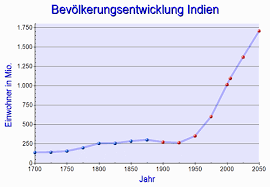
\includegraphics[width=0.48\textwidth]{../99_Bilder/04_Skr_BevInd.png}\\
		\footnotesize{\texttt{Bevölkerungsentwicklung Indien}}\\
		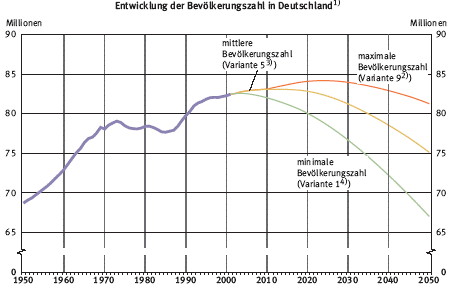
\includegraphics[width=0.48\textwidth]{../99_Bilder/04_Skr_BevDeu.png}\\
		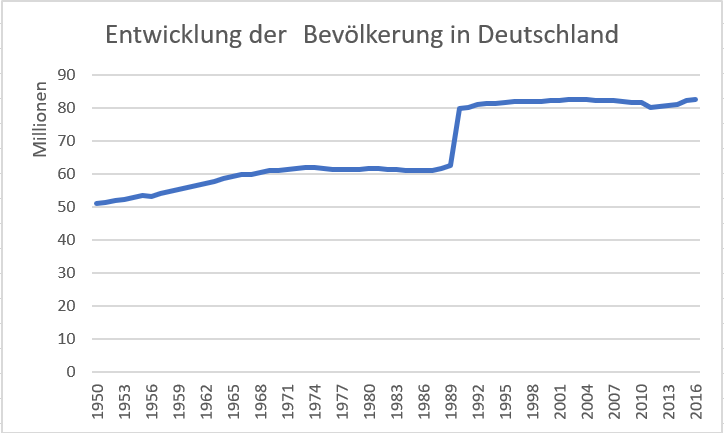
\includegraphics[width=0.48\textwidth]{../99_Bilder/04_Skr_BevDeu2.png}\\
		\footnotesize{\texttt{Bevölkerungsentwicklung für Deutschland. Bis 1989: Früheres Bundesgebiet}}\\
		\normalsize
		\par\noindent
		\subsection*{Beispiel 2: Schulden in Deutschland}
		Genauso kann es neben den absoluten Schuldenwerten interessant sein, die Schuldenentwicklung (also die Neuverschuldung zu verschiedenen Zeitpunkten) zu betrachten.\\
		\par\noindent
		\begin{tabularx}{0.48\textwidth}{|M|M|}
			\hline
			\textbf{Jahr} & \textbf{Schuldenstand in}\\
			0 = 1990; in Jahren & \textbf{Mrd.}\\
			\hline
			0 & 600\\
			\hline
			5 & 1.018\\
			\hline
			10 & 1.210\\
			\hline
			15 & 1.489\\
			\hline
			20 & 2.011\\
			\hline
			25 & 2.000\\
			\hline
		\end{tabularx}
		\subsection{Die \underline{durchschnittliche} Änderungsrate \underline{über einem Intervall \(\lbrack{}x_0;x_1\rbrack\)}}
		Als \textbf{durchschnittliche Änderungsrate} über einem Intervall bezeichnet man die Maßzahl für die Veränderung in einem Zeitraum / Intervall.\\
		Sie kann als \textbf{Quotient} aus dem \textbf{absoluten Zuwachs über einem Intervall} der Länge des Intervalls verstanden werden.
		\[m_{[x_0;x_1]} = \frac{f(x_1) - f(x_0)}{x_1 - x_0}\]
		In einem Graphen kann man diesen Quotienten als \textit{Steigung} der Sekante durch die Punkte \(P(x_0|f(x_0))\) und \(Q(x_1|f(x_1))\) verstanden werden.\\
		\rule{0.48\textwidth}{0.1pt}
		\texttt{\textbf{Wie bestimmt man also die durchschnittliche Änderungsrate über einem bestimmten Intervall?}}\\
		Um diese Frage zu beantworten, schauen wir uns die folgende Funktion und den dazugehörigen Graphen an:\\
		\(f(x) = x^3 - 4x - 1\)\\
		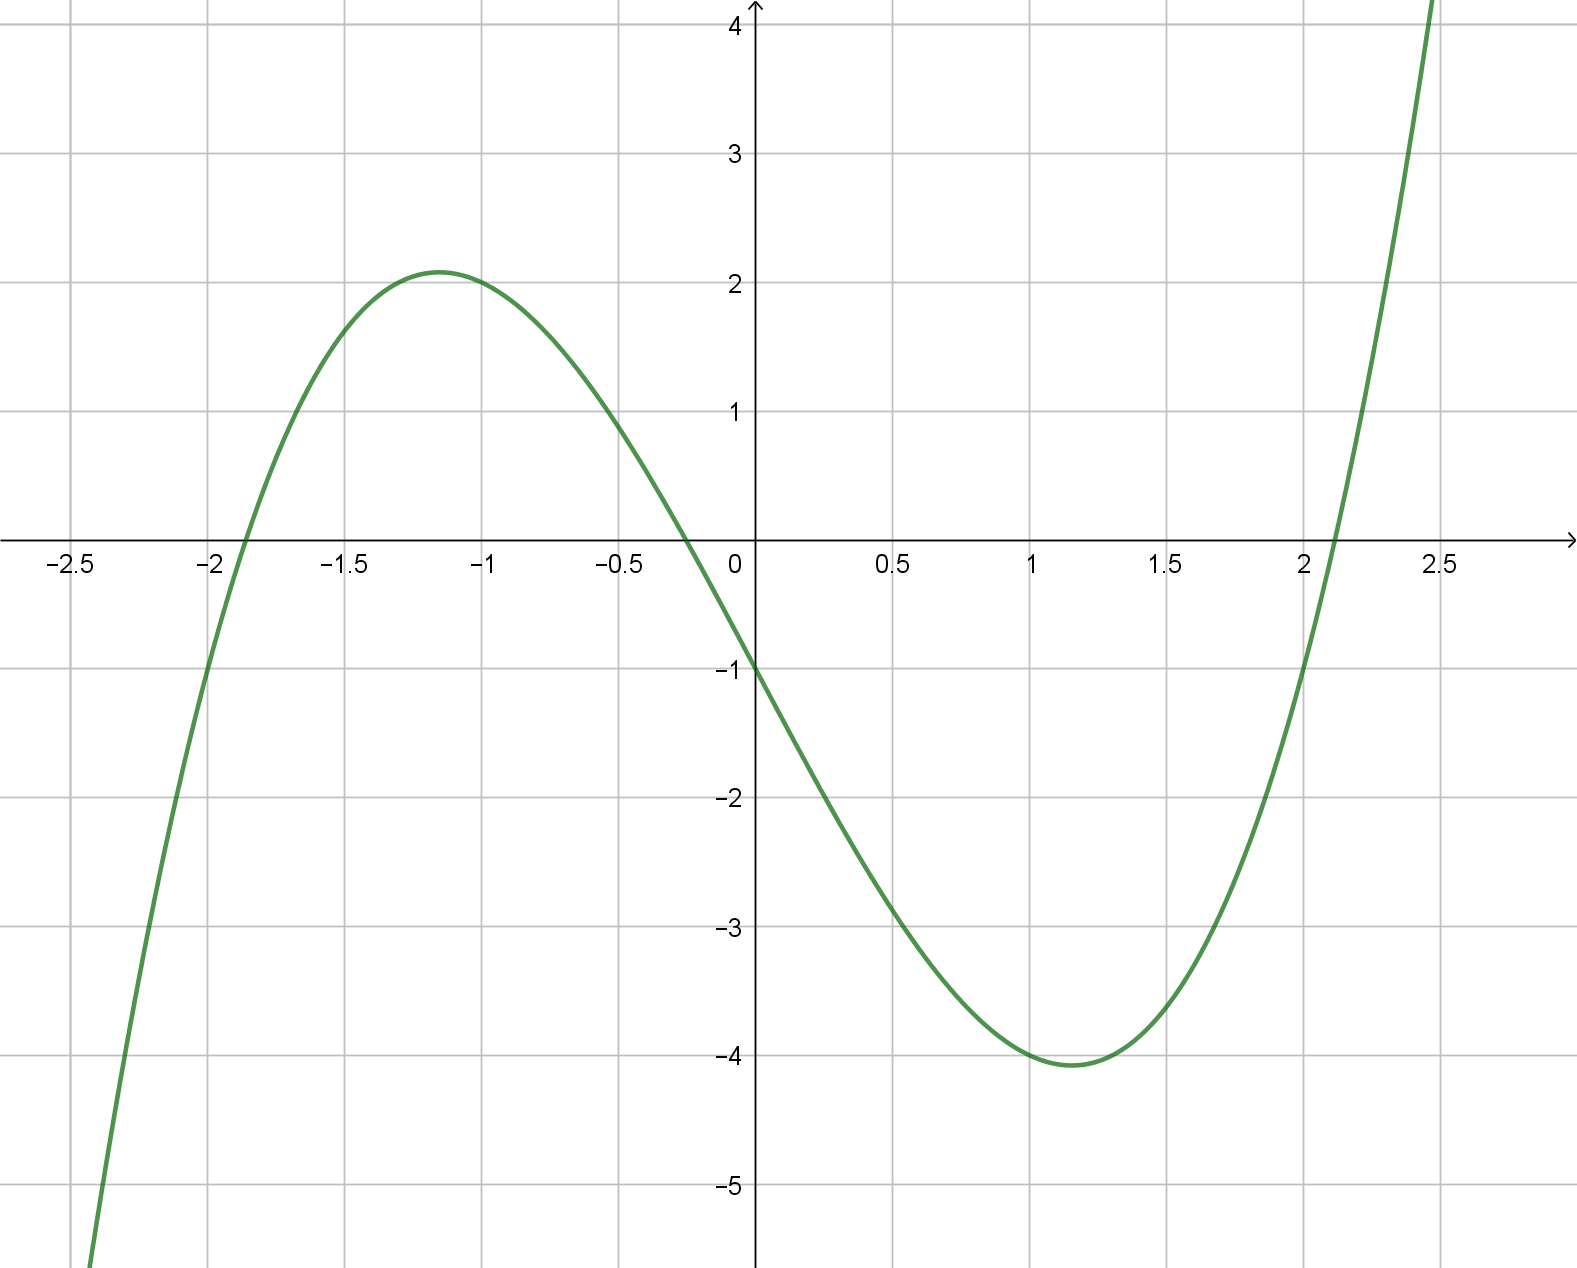
\includegraphics[width=0.48\textwidth]{../99_Bilder/04_Skr_DQFkt.png}\\
		\par\noindent
		Wir möchten versuchen für drei Intervalle die durchschnittliche Änderungsrate zu bestimmen.\\
		\par\noindent
		Zunächst betrachten wir das Intervall \([-2;0]\). Im Graphen können wir die zugehörigen Punkte markieren und anschließend eine Gerade durch beide Punkte\footnote{Sekante} zeichnen.\\
		\par\noindent
		\begin{minipage}{0.2\textwidth}
			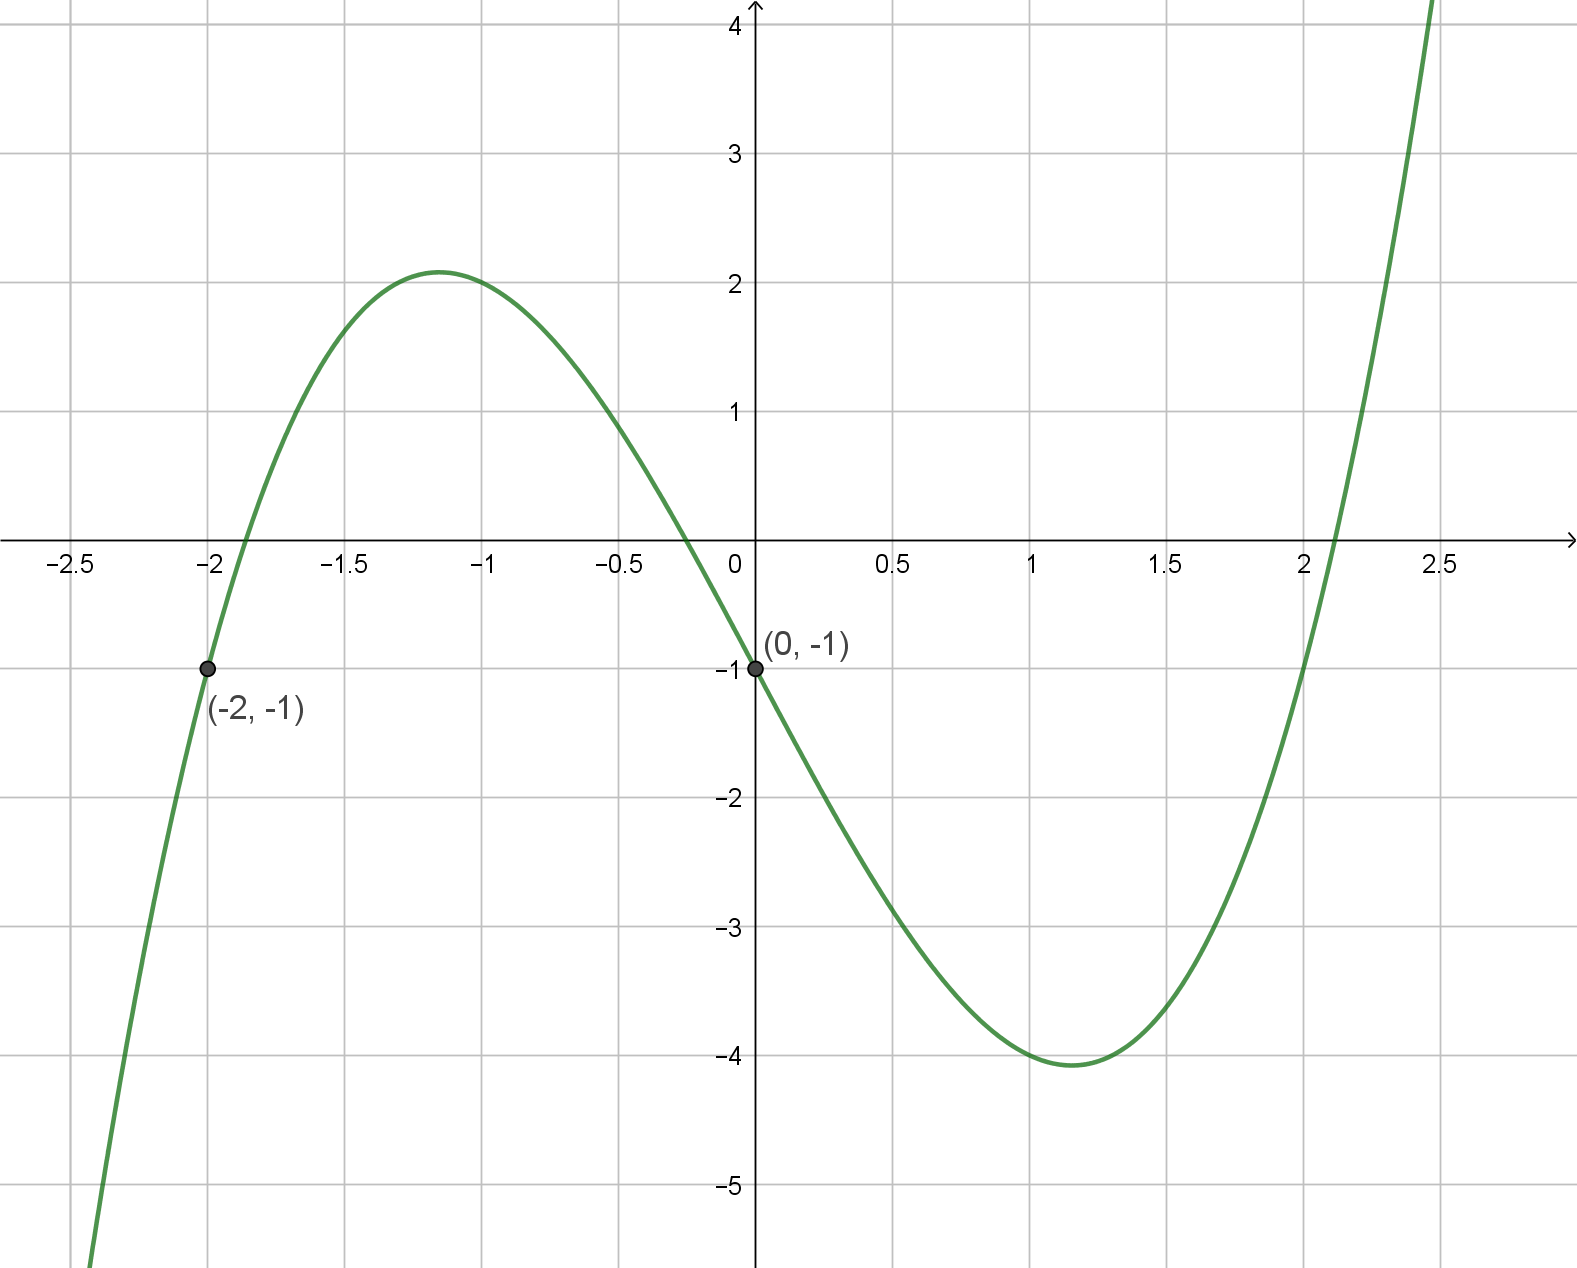
\includegraphics[width=0.98\textwidth,align=t]{../99_Bilder/04_Skr_DifQuo.png}
		\end{minipage}
		\hfill
		\begin{minipage}{0.2\textwidth}
			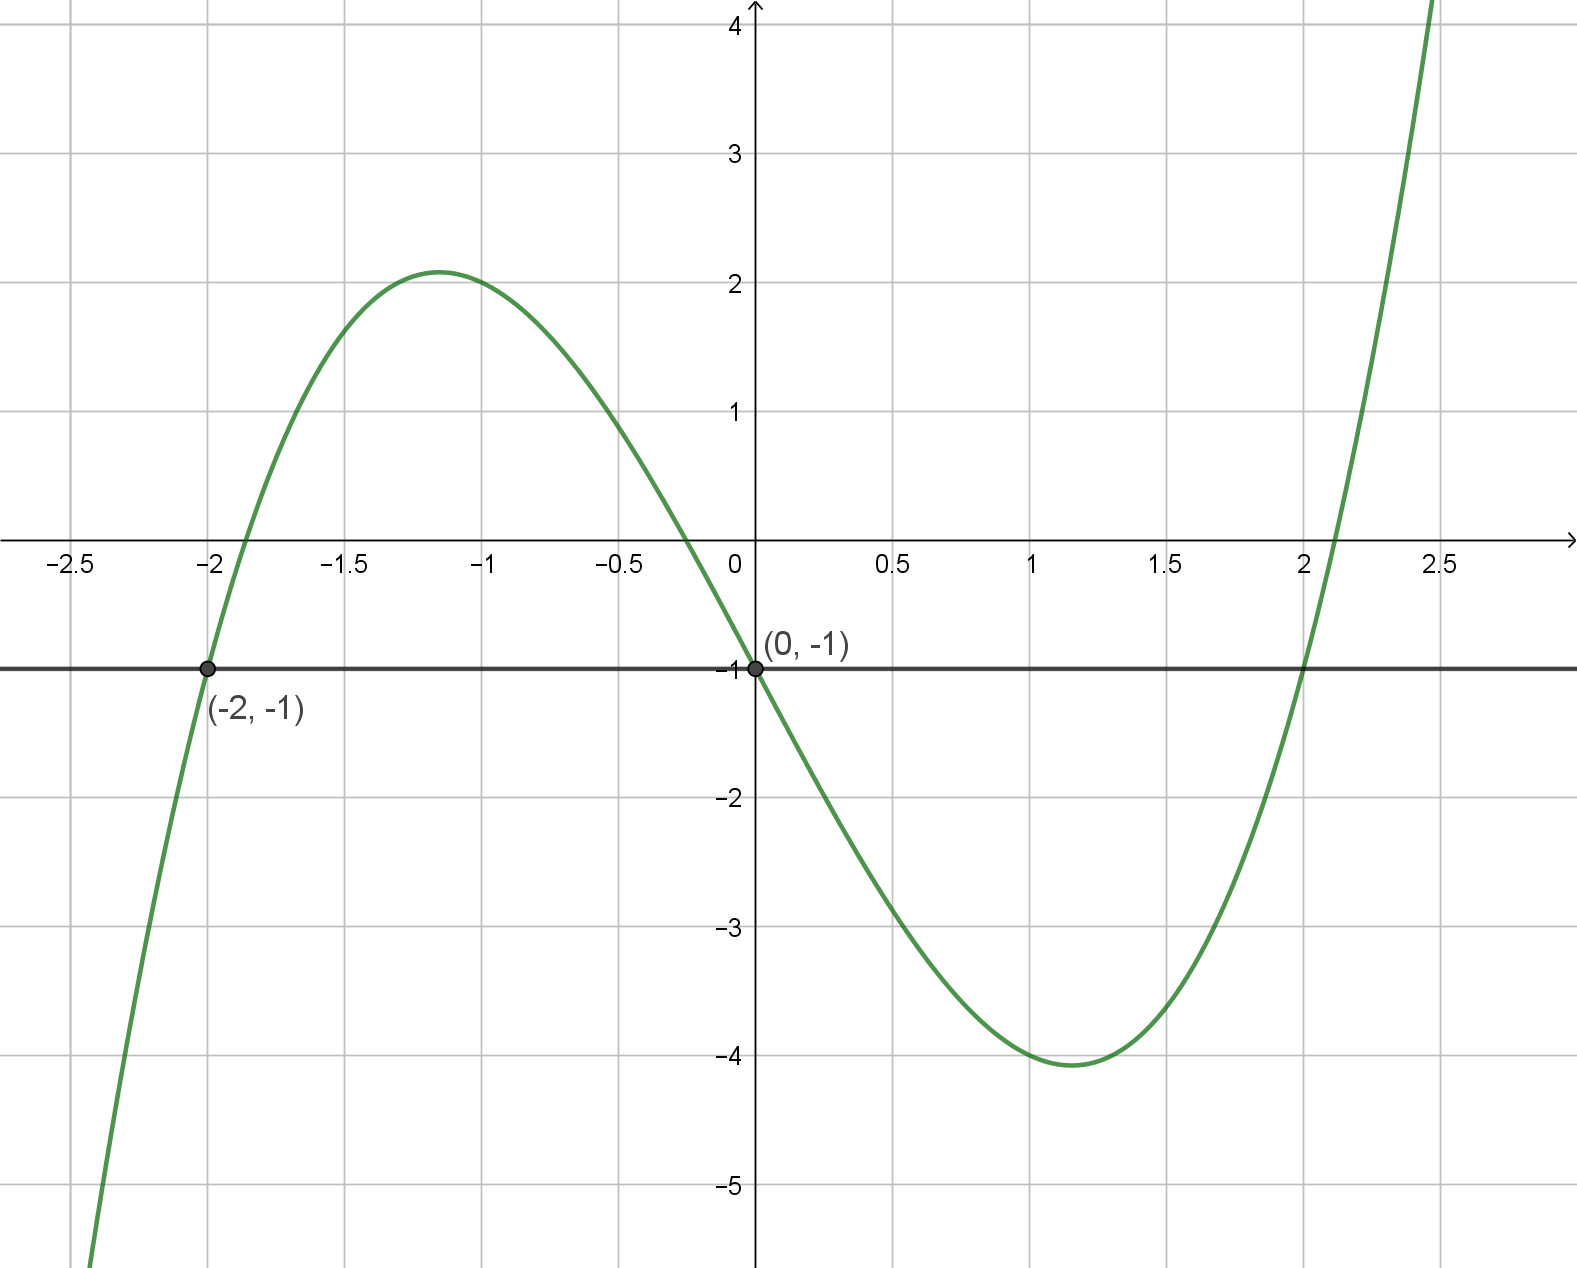
\includegraphics[width=0.98\textwidth,align=t]{../99_Bilder/04_Skr_DifQuo_G.png}
		\end{minipage}\\
		\par\noindent
		Wir haben die Punkte \(P(-2|-1)\) und \(Q(0|-1)\). Für die durchschnittliche Änderungsrate \(m_{[x_0;x_1]}\) ergibt sich somit
		\[m_{[-2;0]} = \frac{\overbrace{(-1)}^{f(x_1)} - \overbrace{(-1)}^{f(x_0)}}{\underbrace{0}_{x_1} - \underbrace{(-2)}_{x_0}} = 0\]
		Über dem Intervall \([-2;0]\) hat die durchschnittliche Änderungsrate den Wert \(0\).\\
		\par\noindent
		Wie sieht es hingegen auf dem Intervall \([0;1]\) aus?\\
		Auch hier markieren wir die zwei Punkte und zeichnen die Sekante durch diese.\\
		\par\noindent
		\begin{minipage}{0.2\textwidth}
			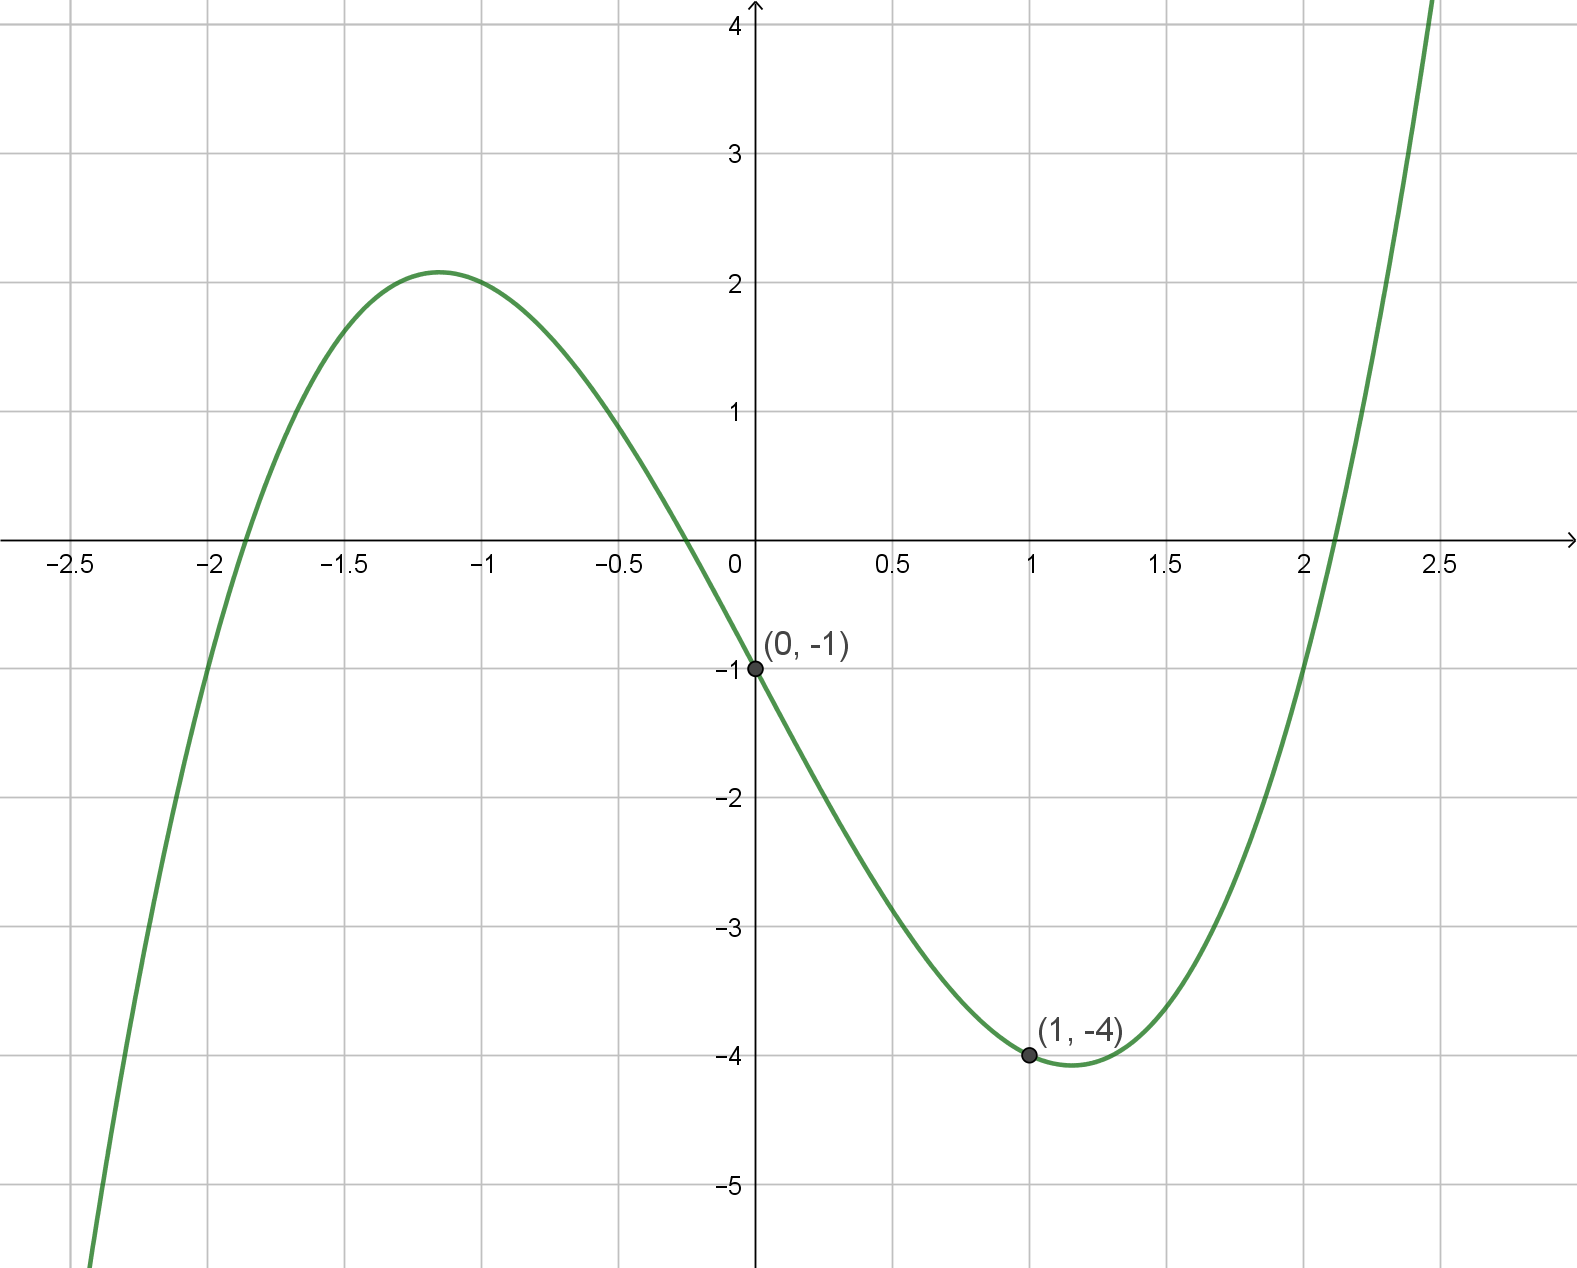
\includegraphics[width=0.98\textwidth,align=t]{../99_Bilder/04_Skr_DifQuo1.png}
		\end{minipage}
		\hfill
		\begin{minipage}{0.2\textwidth}
			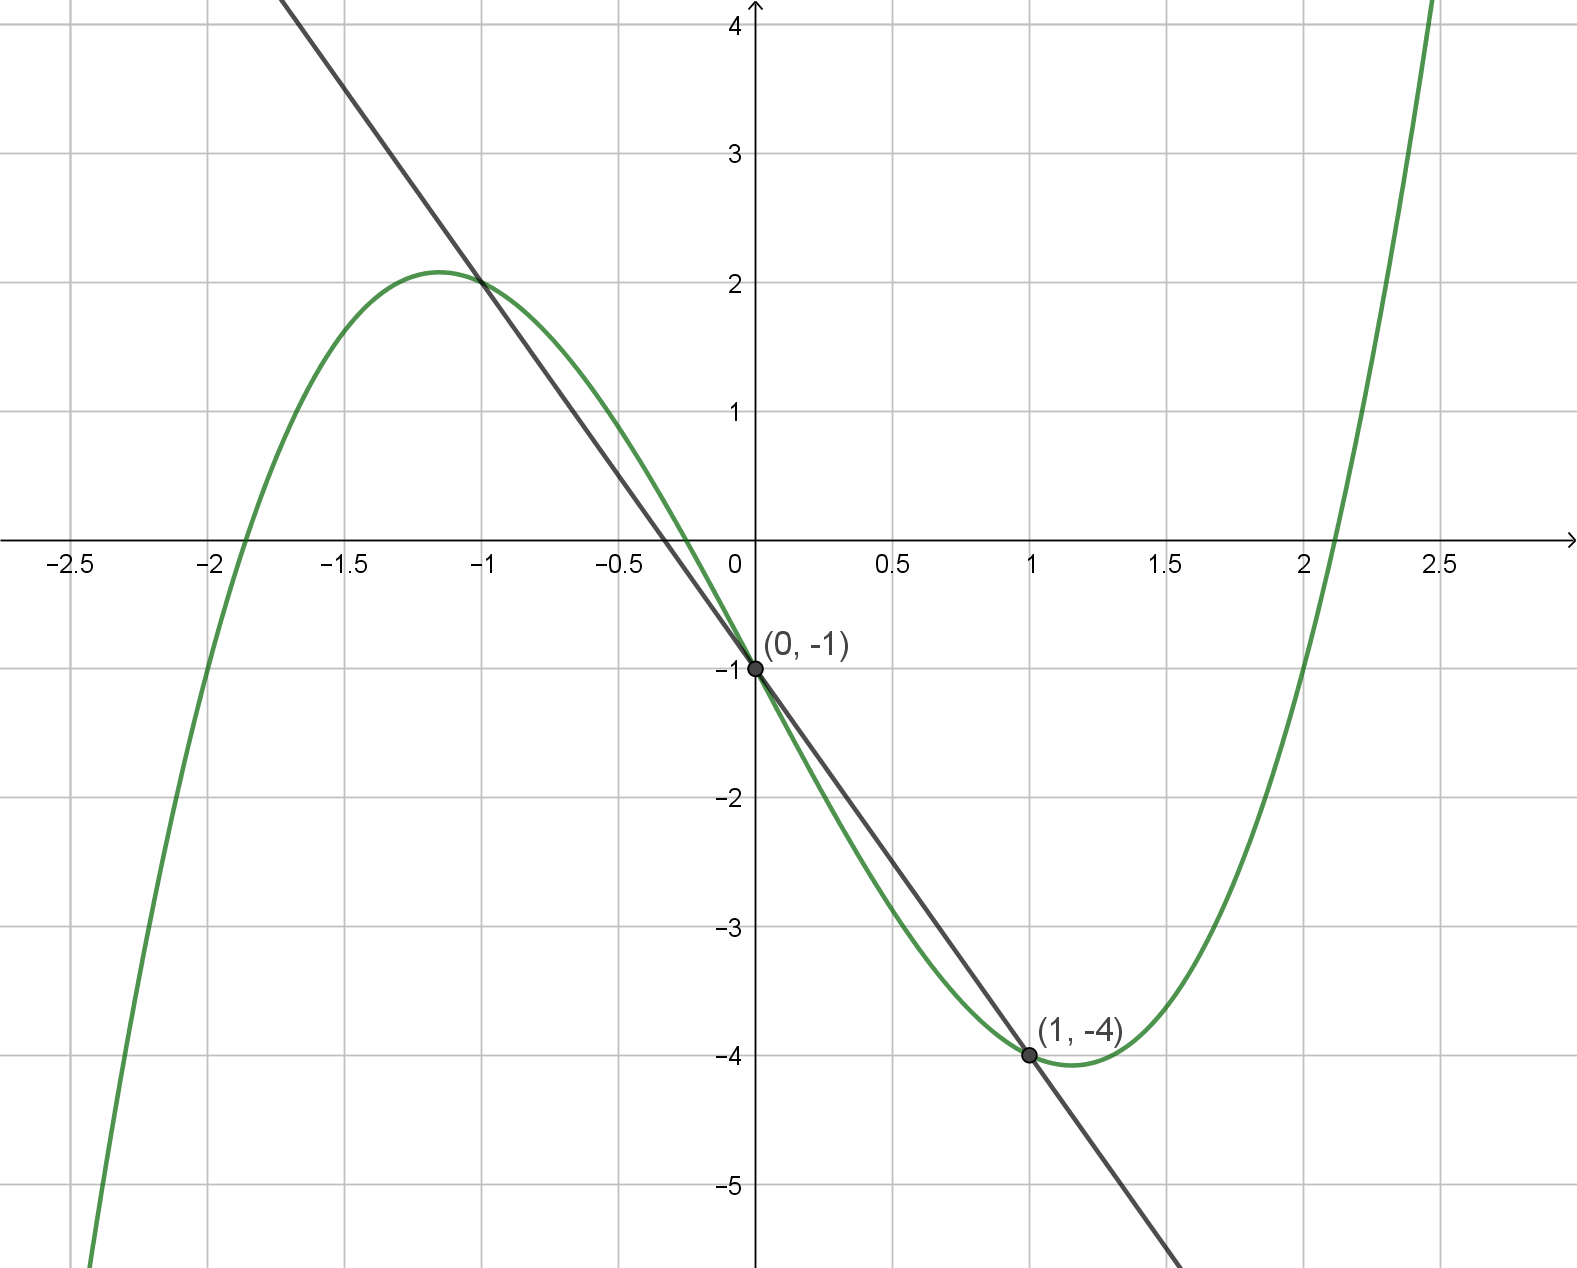
\includegraphics[width=0.98\textwidth,align=t]{../99_Bilder/04_Skr_DifQuo1_G.png}
		\end{minipage}\\
		\par\noindent
		Die zugehörigen Punkte sind \(Q(0|-1)\) und \(R(1|-4)\). Daraus ergibt sich für die durchschnittliche Änderungsrate
		\[m_{[0;1]} = \frac{\overbrace{(-4)}^{f(x_1)} - \overbrace{(-1)}^{f(x_0)}}{\underbrace{1}_{x_1} - \underbrace{(0)}_{x_0}} = -3\]
		über einer Länge von einer Einheit, nimmt der Funktionswert im Durchschnitt um \(3\) ab.\\
		\par\noindent
		Betrachten wir zu guter Letzt noch das Intervall \([1;2]\).\\
		\par\noindent
		\begin{minipage}{0.2\textwidth}
			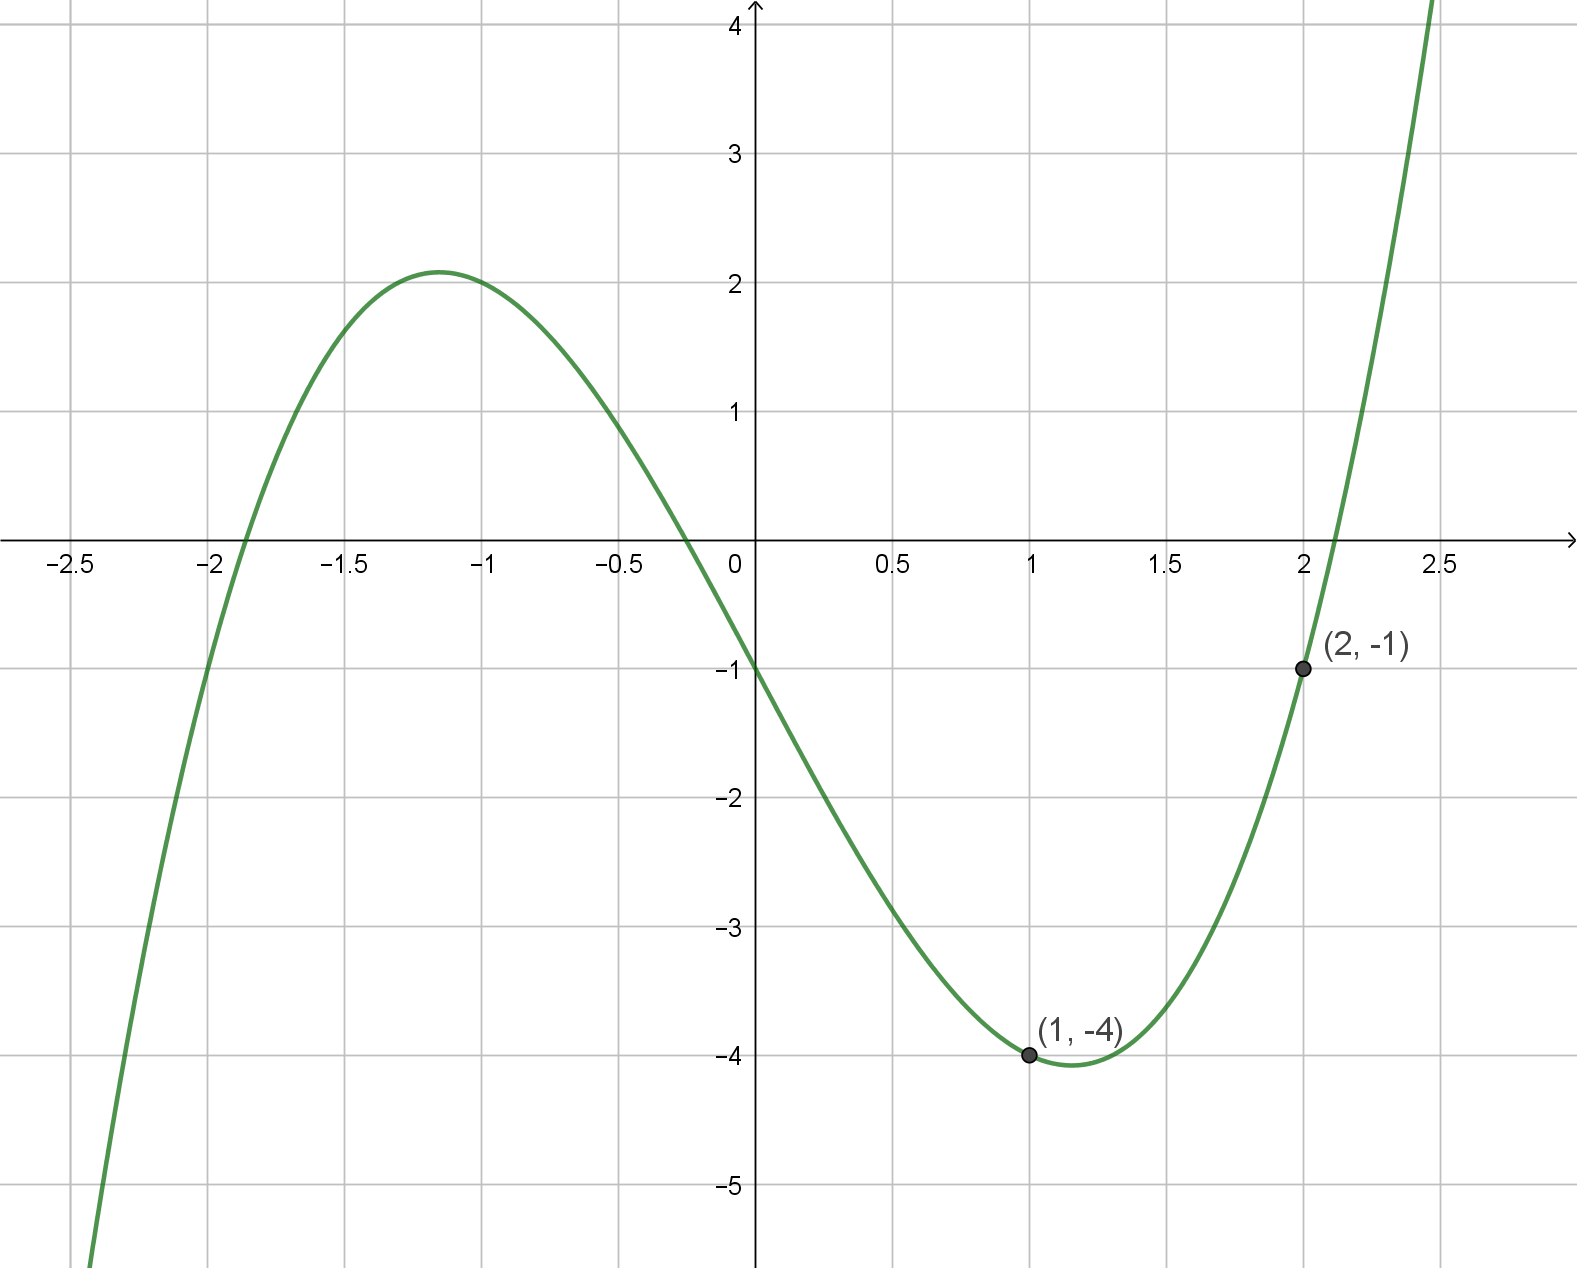
\includegraphics[width=0.98\textwidth,align=t]{../99_Bilder/04_Skr_DifQuo2.png}
		\end{minipage}
		\hfill
		\begin{minipage}{0.2\textwidth}
			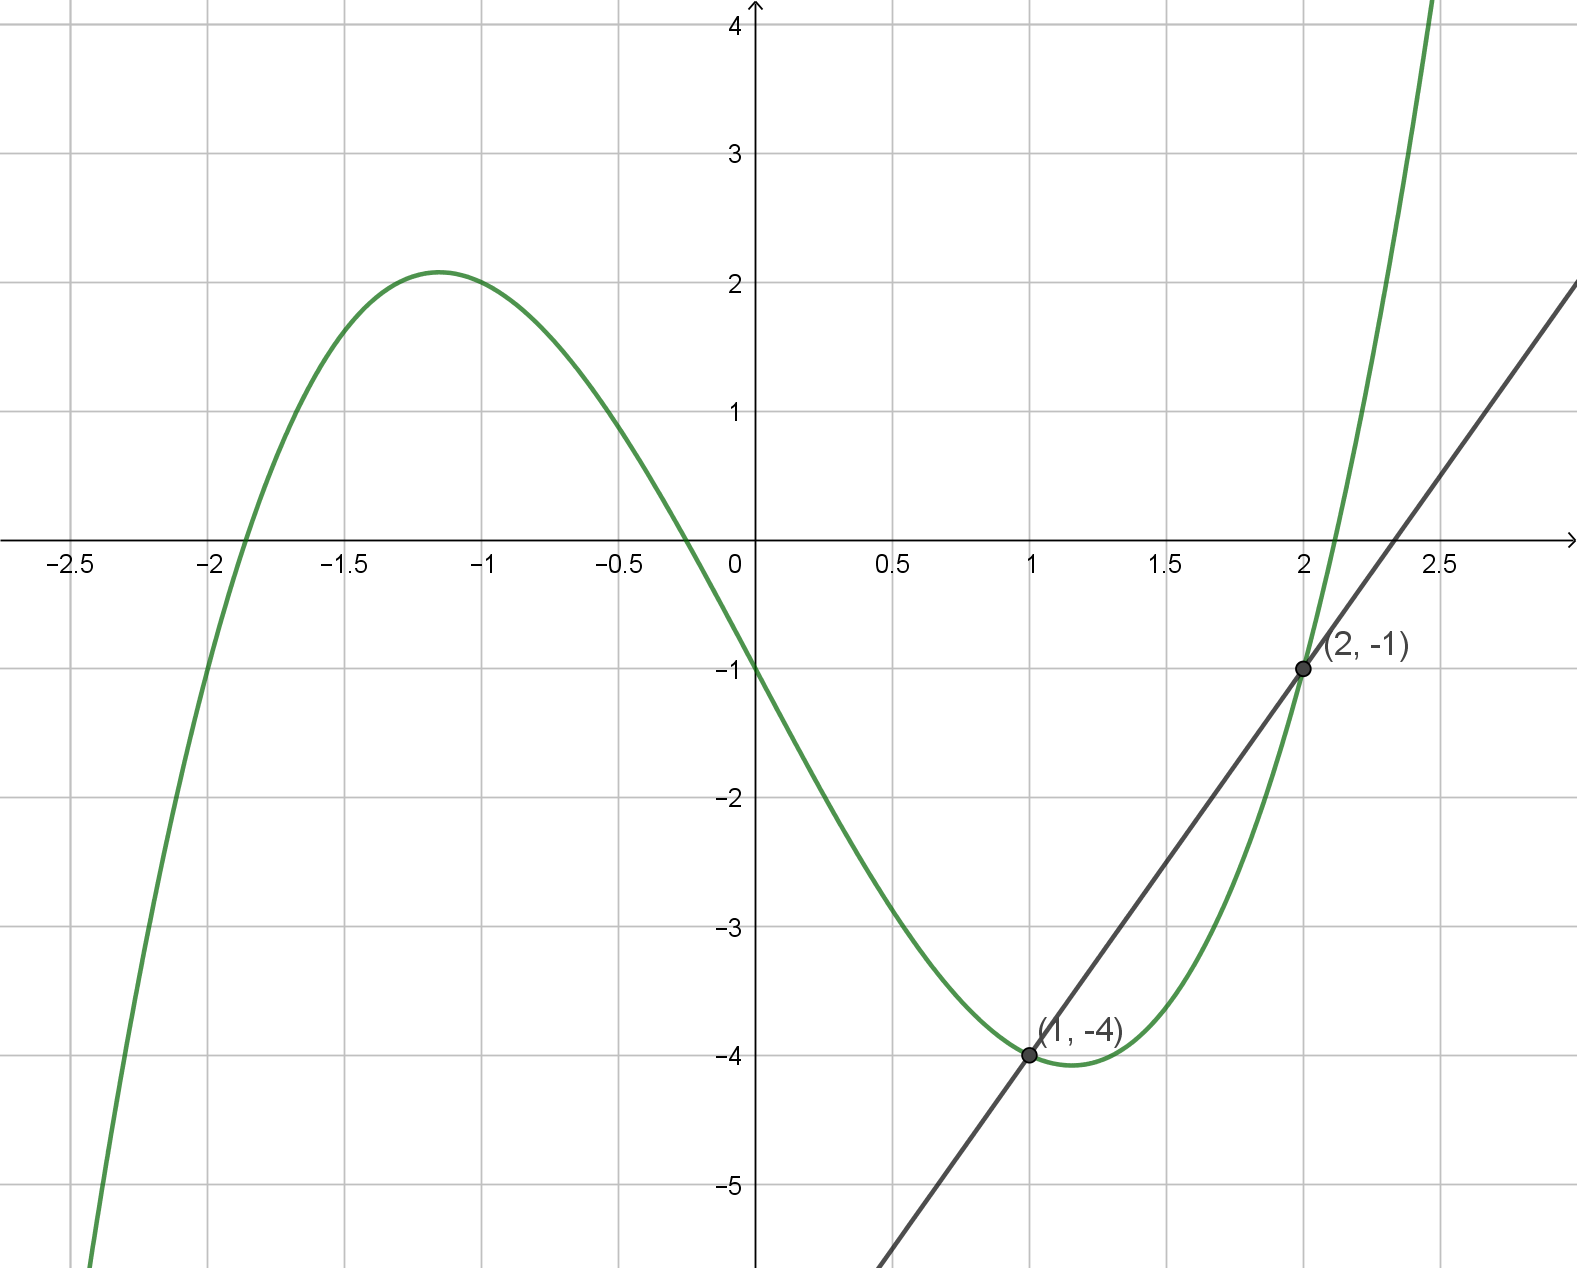
\includegraphics[width=0.98\textwidth,align=t]{../99_Bilder/04_Skr_DifQuo2_G.png}
		\end{minipage}\\
		\par\noindent
		Die entsprechenden Punkte sind \(R(1|-4)\) und \(S(2|-1)\). Somit haben wir eine durchschnittliche Änderungsrate von
		\[m_{[1;2]} = \frac{\overbrace{(-1)}^{f(x_1)} - \overbrace{(-4)}^{f(x_0)}}{\underbrace{2}_{x_1} - \underbrace{(1)}_{x_0}} = 3\]
		Mit diesem Wert können wir also festhalten, dass über eine Länge von einer Einheit der Funktionswert im Durchschnitt um \(3\) zunimmt.\\
		\subsubsection{Übung}
		\begin{enumerate}
			\item Berechnen Sie die Durchschnittlichen Änderungsraten zu den im ersten Kapitel gegebenen Entwicklungen für folgende Intervalle:
			\begin{itemize}[label=-]
				\item Bevölkerungsentwicklung Indien \([2010;2050]\)
				\item Bevölkerungsentwicklung Deutschland \([2010;2050]\)
				\item Bevölkerungsentwicklung Deutschland \([2010;2040]\)
				\item Bevölkerungsentwicklung Deutschland \([2010;2020]\)
				\item Bevölkerungsentwicklung Deutschland \([2010;2011]\)
			\end{itemize}
			\item Welche der zu Deutschland berechneten Wachstumsraten ist am besten geeignet um die \underline{momentane} Wachstumsdynamik zum Zeitpunkt 2010 zum Ausdruck zu bringen?
		\end{enumerate}
		\rule{0.48\textwidth}{0.1pt}
		\subsection*{Vorschau: Von der \underline{durchschnittlichen} Änderungsrate zur \underline{momentanen} Änderungsrate}
		Bei der durchschnittlichen Änderungsrate handelt es sich nur um eine Annäherung an die Dynamik an einer bestimmten Stelle. Da sich aber die Dynamik schnell ändern kann, spielt die Dynamik zu einem bestimmten Zeit\underline{punkt} eine besondere Rolle.\\
		Hierbei spricht man dann von der \textbf{momentanen Änderungsrate}.
		\subsubsection*{Beispiel 1: Radarkontrolle}
		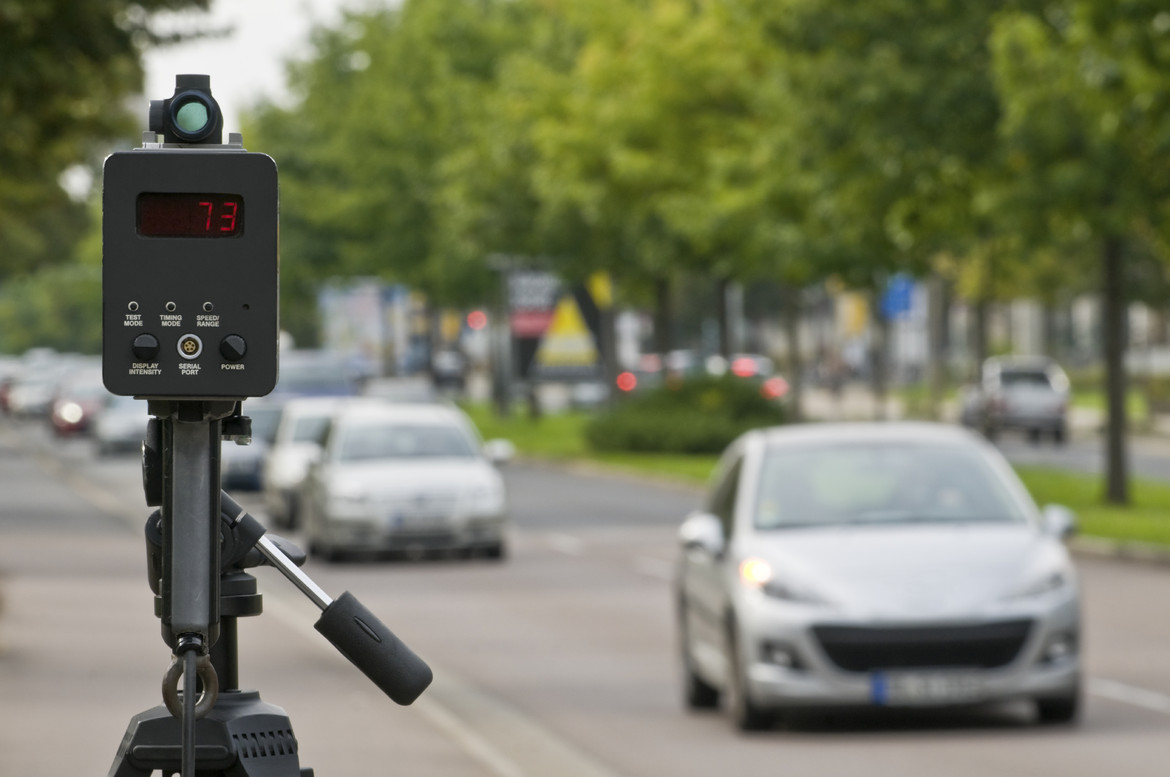
\includegraphics[width=0.48\textwidth]{../99_Bilder/04_Skr_momAen.jpg}\\
		Bei der Radarkontrolle wird nicht die durchschnittliche Geschwindigkeit über eine bestimmte Zeit gemessen, sondern lediglich die Geschwindigkeit zu einem bestimmten Zeitpunkt.\\
		Das heißt, selbst wenn über einen Zeitraum von 10 Minuten die durchschnittliche Geschwindigkeit bei \(50 \frac{km}{h}\) liegt, kann die momentane Geschwindigkeit erheblich abweichen (z.B \(70 \frac{km}{h}\)).\footnote{Vergleiche hierzu: Mathematik Technik - Fachhochschulreife S. 130. Beispiel 4 Radarkontrolle.}
		\subsubsection*{Beispiel 2: Fallschirmsprung}
		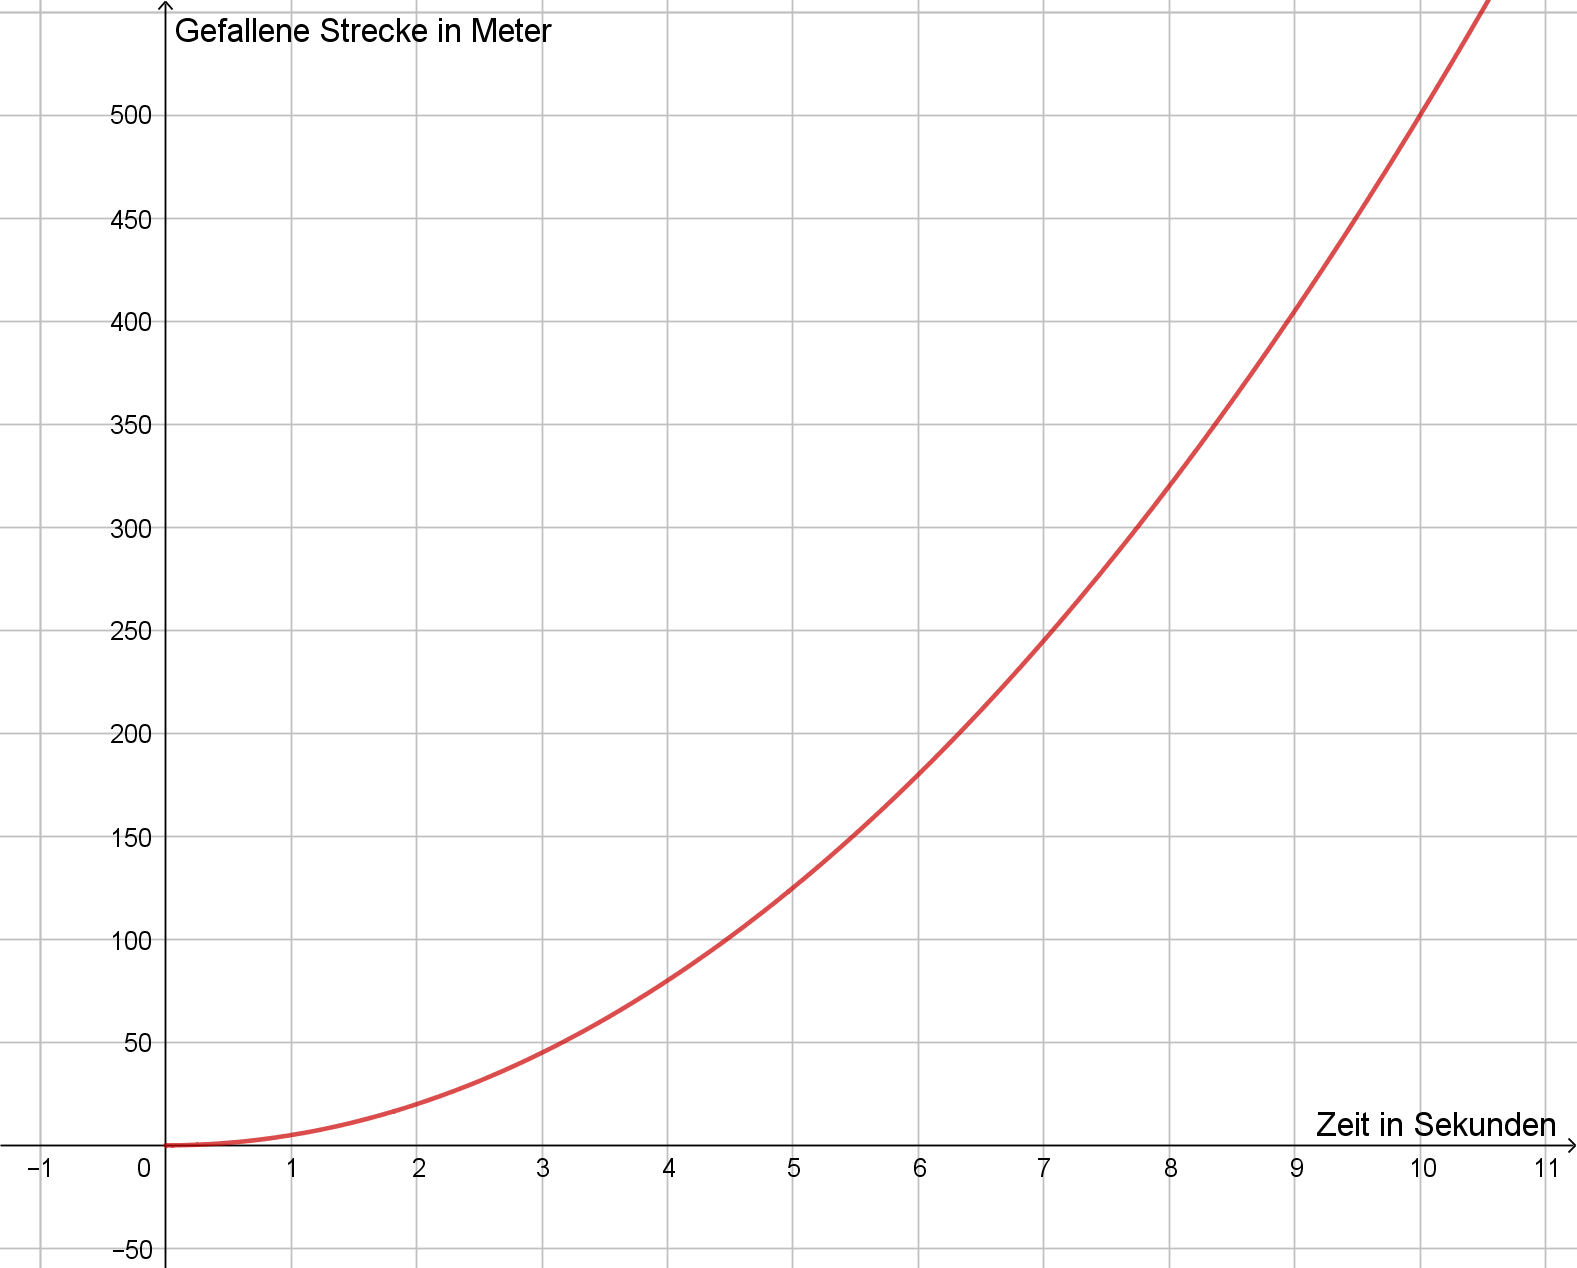
\includegraphics[width=0.48\textwidth]{../99_Bilder/04_Skr_FallS.jpg}\\
		Ähnlich wie bei der Radarkontrolle kann man auch die Geschwindigkeit bei einem Fallschirmsprung messen.
		\subsubsection*{Die Bestimmung der \underline{momentanen} Änderungsrate \underline{an einer Stelle \(x_0\)}}
		Die durchschnittliche Änderungsrate kann nur ein ungefähres Bild der tatsächlichen Dynamik bzw. Steigung an einem bestimmten Punkt liefern. Je größer das Intervall ist, für welchen die Dynamik betrachtet wird, umso schlechter kann die Realität dargestellt werden.\\
		\par\noindent
		Somit müssen wir versuchen, die Steigung in einem Punkt anzunähern. Dies können wir tun, indem wir das Intervall über dem wir die Dynamik bestimmen immer kleiner werden lassen.\\
		\par\noindent
		Ähnlich wie bei der durchschnittlichen Änderungsrate spricht man auch in diesem Fall von der Änderungsrate. Da wir diese aber in einem bestimmten Punkt angeben, bezeichnet man sie aber als \textbf{momentane Änderungsrate}.\\
		\par\noindent
		\texttt{Wie könnte man diese nun bestimmen?}\\
		Zu dem bestimmten Zeitpunkt \(x_0\) wählen wir einen weiteren Punkt \(x_1 = x_0 + h\) und erhalten so das Intervall \(I = [x_0; \underbrace{x_0 + h}_{x_1}]\).\\
		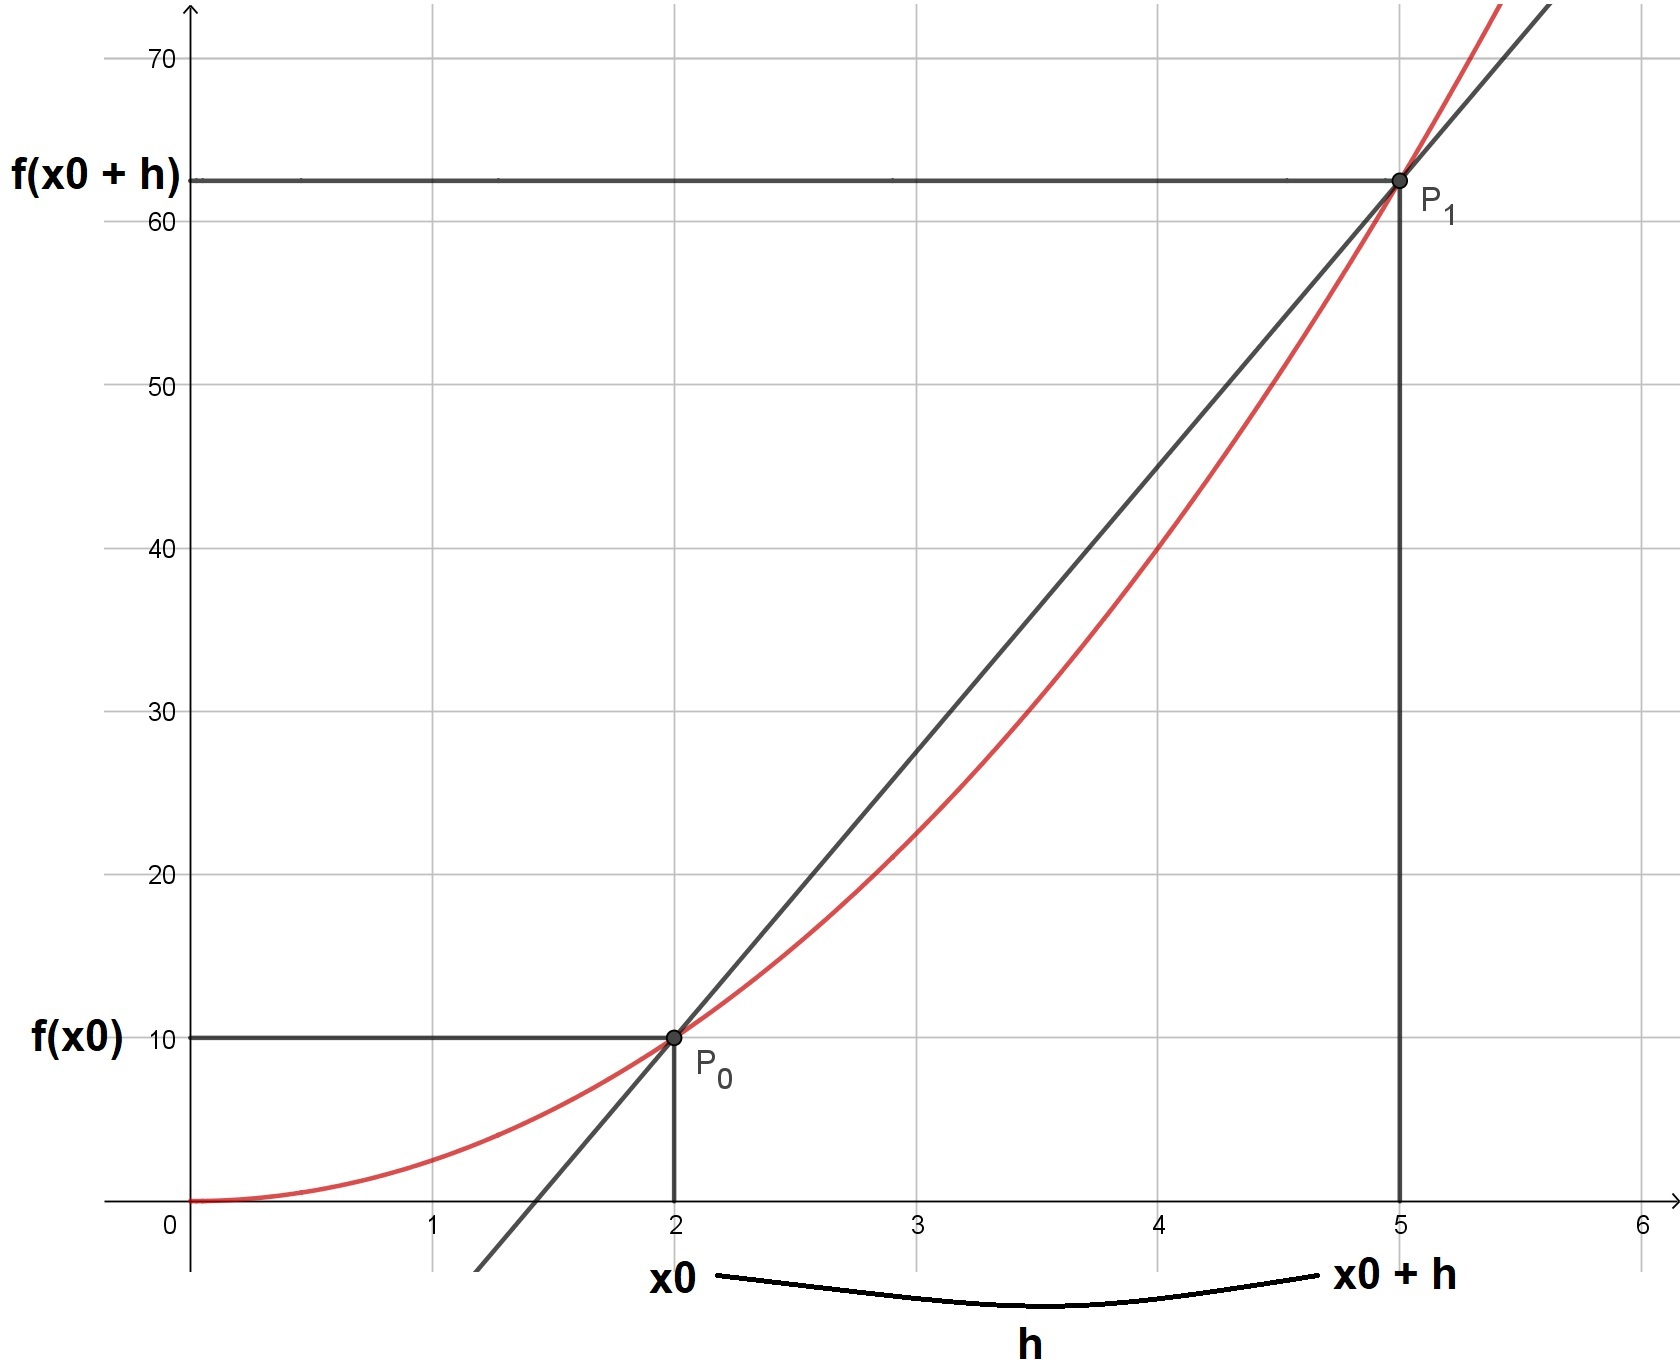
\includegraphics[width=0.48\textwidth]{../99_Bilder/04_Skr_DiffQuo.jpg}\\
		\par\noindent
		Die eingezeichnete Sekante hat die Steigung
		\[m_{[x_0;x_0+h]} = \frac{f(x_0-h) - f(x_0)}{h}\]
		Verändern wir nun \(h\) so, dass das Intervall immer kleiner wird\footnote{Also \(h\rightarrow{}0\).}, nähern wir uns mit der Sekante immer mehr an die Tangente im Punkt \(x_0\) an.
	\end{worksheet}
\end{document}